\synctex=1
\documentclass[12pt,a4paper,oneside]{article}

\usepackage[spanish]{babel}

\usepackage{fancyhdr}
\usepackage{geometry}
\usepackage{graphicx}
\usepackage{wrapfig}
\usepackage{lastpage}
\usepackage[hidelinks]{hyperref}
\usepackage{authblk}
\usepackage{bookmark}

\usepackage[utf8]{inputenc} % Required for inputting international characters
\usepackage[T1]{fontenc} % Output font encoding for international characters
\usepackage{mathpazo} % Palatino font

\makeatletter
\newcommand{\subtitledoc}[1]{\newcommand{\@subtitledoc}{#1}}
\newcommand{\instituto}[1]{\newcommand{\@instituto}{#1}}
\newcommand{\carrera}[1]{\newcommand{\@carrera}{#1}}
\newcommand{\professor}[1]{\newcommand{\@professor}{#1}}
\newcommand{\catedraCaratula}[1]{\newcommand{\@catedraCaratula}{#1}}
\newcommand{\catedraHeader}[1]{\newcommand{\@catedraHeader}{#1}}
\newcommand{\curso}[1]{\newcommand{\@curso}{#1}}
\newcommand{\legajo}[1]{\newcommand{\@legajo}{#1}}
\newcommand{\footerauthor}[1]{\newcommand{\@footerauthor}{#1}}
\newcommand{\footerlegajo}[1]{\newcommand{\@footerlegajo}{#1}}

%Configuracion de hoja (margenes y tamaño)
\geometry{a4paper,margin=1in}
\setlength\headheight{28pt}

%formato de encabezado y pie para todas las paginas.
\fancyhead[L]{
    \begin{minipage}[b]{7.5mm}
        
\includegraphics[width=7mm]{Imagenes/logo-utn.png}
    \end{minipage}
    \begin{minipage}[b]{90mm}
        \textbf{Alumnos: }\@footerauthor \\
        \textbf{Legajos: }\@footerlegajo
    \end{minipage}
}
\fancyhead[R]{
    \textbf{Curso:} \@curso\\
    \textbf{Cátedra:} \@catedraHeader
}
\fancyfoot[L]{\@date}
\fancyfoot[C]{} %eliminar antiguo numero de pagina
\fancyfoot[R]{Página \thepage\ de \pageref{LastPage}}
\renewcommand{\headrulewidth}{0.5pt}
\renewcommand{\footrulewidth}{0.5pt}
\pagestyle{fancy}

\addto\captionsspanish{%
	\renewcommand{\contentsname}%
	{CONTENIDO}%
}

\renewcommand{\maketitle}{%
    \newpage
    \thispagestyle{empty}
    
    \begin{center}

    \textsc{\LARGE \@instituto}\\[0.5cm] 
    \textsc{\Large \@carrera}\\[1.5cm] 
    
\includegraphics[width=0.30\textwidth]{Imagenes/logo-utn.png} \par
    \vspace{1.5cm}
    
    \textsc{\large \@catedraCaratula }\\[0.5cm]
    
    {\huge\bfseries \@title}\\[0.4cm]
    \textsc{\Large \@subtitledoc}\\[0.5cm]
    

    \end{center}

    \vspace{2cm}

    {\noindent
    \begin{minipage}[t]{.2\textwidth}
        \raggedright
        \textbf{ALUMNOS} \par
        ~\\
        ~\\
        ~\\
        \textbf{CURSO} \par
        ~\\
        \textbf{DOCENTES} \par
        \end{minipage}%
     \begin{minipage}[t]{.05\textwidth}
        \raggedright
        \textbf{:} \par
        ~\\
        ~\\
        ~\\
        \textbf{:} \par
        ~\\
        \textbf{:} \par
    \end{minipage}%
    \begin{minipage}[t]{.55\textwidth}
        \raggedright
        \@author \par
        ~\\
        \@curso \par
        ~\\
        \@professor \par
        ~\\
    \end{minipage}%
    \begin{minipage}[t]{.15\textwidth}
        \raggedright
        \@legajo \par
    \end{minipage}
    }
    \vfill
    \begin{center}
        \textbf{CÓRDOBA, ARGENTINA} \par
        \textbf{\@date}
    \end{center}
    \newpage
}

\makeatother


\instituto{Universidad Tecnológica Nacional\\[0.2cm]Facultad Regional Córdoba}
\carrera{Ingeniería Electrónica}
\title{Trabajo Práctico de Laboratorio Nº6}
\subtitledoc{MEDICIÓN DE POTENCIA ACTIVA Y DE FACTOR DE POTENCIA CON OSCILOSCOPIO}
\professor{Ing. Centeno, Carlos \par Ing. Salamero, Martin \par Ing. Guanuco, Luis}
\catedraCaratula{Medidas Electrónicas I}
\catedraHeader{Med. Electrónicas I}
\curso{4R1}
\author{Carreño Marin, Sebastian \par Juarez, Daniel \par Torres, Heber}
\legajo{83497 \par 79111 \par 84640}
\footerauthor{Carreño Marin, Juarez, Torres}
\footerlegajo{83497, 79111, 84640}
%\date{\the\year}
\date{4 de agosto de 2022}



\usepackage{float}
\usepackage{amsmath}
\usepackage{amssymb}
\usepackage{booktabs}
\usepackage{multirow} 
\usepackage{siunitx}
\usepackage{caption}
\usepackage{subcaption}
\usepackage{blindtext}
\usepackage{multicol}
\usepackage{enumerate}
\usepackage{mathtools}
\usepackage{array}
\usepackage{soul}
\usepackage{booktabs}
\usepackage{svg}

\usepackage[spanish]{babel} \addto\captionsspanish{\def\tablename{Tabla}   
\def\listtablename{\'Indice de tablas} } 





\begin{document}
  \maketitle

  \null
  \thispagestyle{empty}
  \pagebreak

  \setcounter{page}{1}
  \tableofcontents
  \newpage
  %\listoffigures
  %\listoftables
  %\pagebreak
  
  %Introducción del TP%  
\section{Introducción}

   A nivel industrial, la determinacion de frecuencias industriales como la potencia y el factor de potencia se 
   determinan mediante el uso de aparátos de medicion, destinados a medir dichas magnitudes 
   en laboratorios electricos. En el presente trabajo práctico emplearemos metodos de medicion 
   indirectos, e instrumentos utilizados en electronica, como un osciloscopio de uso general, 
   para las mediciones de dichas magnitudes industriales.   


    \section{Marco Teórico}

    \section{Actividad Práctica}
    Se propone realizar las mediciones de \textbf{potencias} y \textbf{factor de potencia}, y posteriormente,
    la \textbf{correción} de dicho factor, en una carga reactiva, la cual se trata de un tubo fluorescente 
    común. Este mismo se encuentra preparado junto a un circuito de medición que provee la cátedra. En la 
    Figura~\ref{fig:CircuitoMedicion} se puede apreciar un esquema del mismo y una foto real.

    \begin{figure}[H]
      \centering
        \begin{subfigure}[t]{\textwidth}
          \centering
          \frame{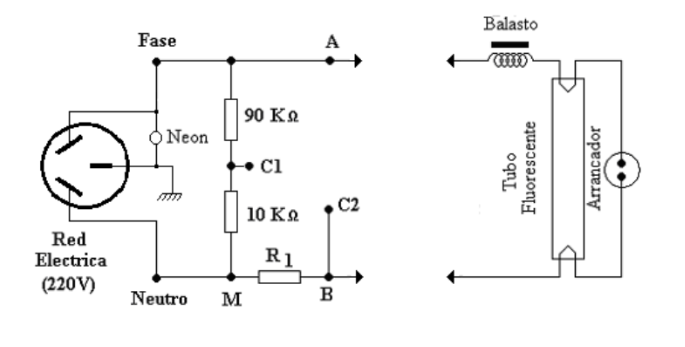
\includegraphics[width=0.7\textwidth]{Imagenes/ActividadPractica/EsquemaCircuito.png}}
          \caption{Esquema.}
          \label{fig:EsquemaCircuito}
        \end{subfigure}
        \begin{subfigure}[t]{\textwidth}
          \centering
          \frame{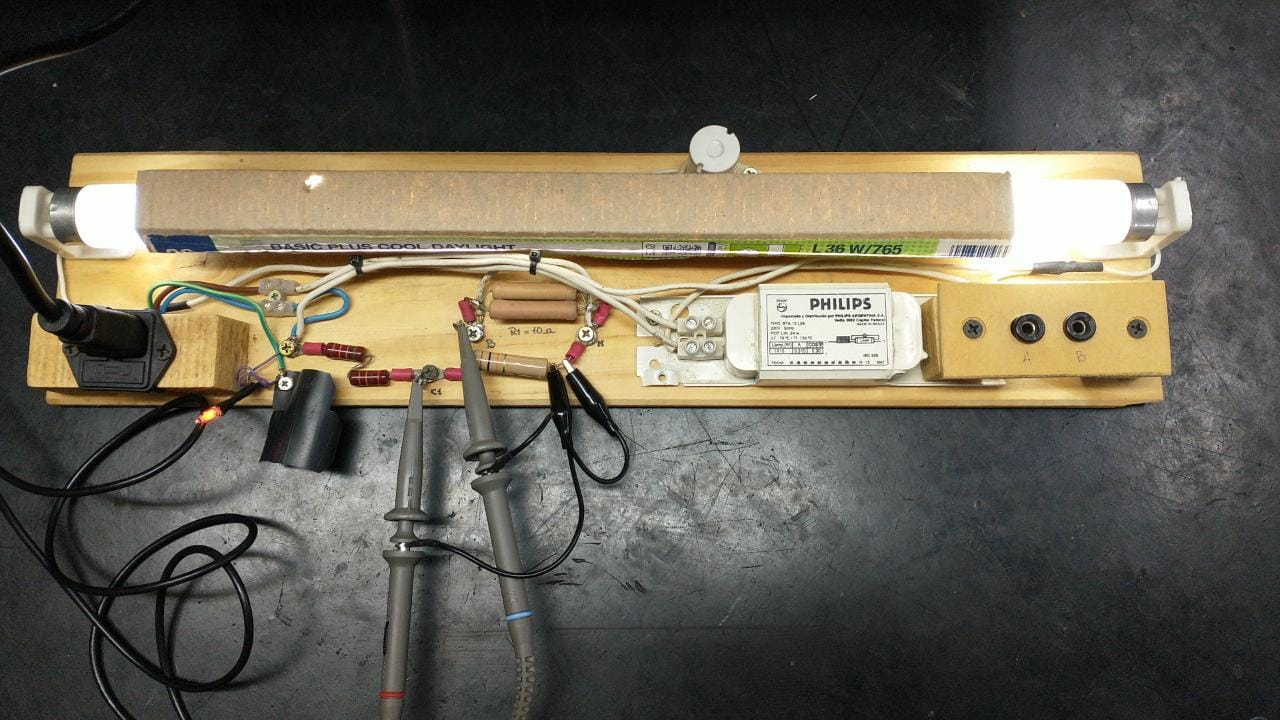
\includegraphics[width=0.7\textwidth]{Imagenes/ActividadPractica/FotoRealCircuito.jpeg}}
          \caption{Foto real.}
          \label{fig:FotoRealCircuito}
        \end{subfigure}
      \caption{Circuito de medición propuesto por la cátedra.}
      \label{fig:CircuitoMedicion}
    \end{figure}

    En el circuito de medición se puede apreciar el punto \textbf{M}, en el cual se conecta la tierra del osciloscopio
    por medio de sus puntas. Por esta razón, es importante y obligatorio el uso de un \textbf{transformador de aislación},
    el cual tiene una de relación 1:1, y tiene como función crear una barrera física de aislación
    entre los equipos/circuitos con los cuales se trabaja y la red. Esto se justifica con que, la diferencia de
    potencial entre \textit{neutro} y \textit{tierra} de la red no es cero (idealmente debería serlo), para este caso, dicho
    valor es de aproximadamente $\mathbf{1,27\ V}$. Este valor generaría un flujo de corriente a través del osciloscopio 
    directo a la \textit{tierra}, lo cual podría dañar el instrumento, y además, provocaría que el diferencial se active.

    Siguiendo con el análisis del circuito de medición, se puede apreciar un divisor resistivo. Esto permite que, en el
    punto \textbf{C1} se pueda medir la \textbf{décima parte} de la tensión de entrada. Luego, en el punto \textbf{C2} 
    se mide la corriente de entrada por Ley de Ohm, ya que el valor de la resistencia es $\mathbf{R_l=10\ \Omega}$.
    
    Se aclara que el kit utilizado no respeta el código de colores de los cables, siendo la fase y el neutro de color azul
    y marrón respectivamente.

      \subsection{Medición de potencia activa y factor de potencia} 
  

      \subsection{Correción del factor de potencia}













    \section{Conclusiones}

  
\end{document}
